\documentclass[aspectratio=43]{beamer}%[handout]
\mode<handout>{
\usepackage{pgfpages}
\pgfpagesuselayout{4 on 1}[letterpaper,border shrink=5mm, landscape]
}
\usepackage[T1]{fontenc}
\usepackage[utf8]{inputenc}
\usepackage[spanish]{babel}
\usepackage{beamerthemeshadow,beamerthemesplit,cite,cancel,lmodern,eso-pic,fancyvrb,textcomp,lmodern,url,times,booktabs,amssymb,amsmath,ragged2e,float,subfig,xspace,epic,eepic,multicol,multirow,colortbl,color,graphicx,url}
\usepackage[normalem]{ulem} %tachar texto con \sout{}
\usepackage{listings} %CODIGOs
\usepackage[sfdefault]{roboto}
\setcounter{tocdepth}{3}
\usepackage[figurename=]{caption}
%Colores Ulagos
\definecolor{gray97}{gray}{.97}
\definecolor{gray75}{gray}{.75}
\definecolor{gray45}{gray}{.45}
\definecolor{listinggray}{gray}{0.9}
\definecolor{lbcolor}{rgb}{0.9,0.9,0.9}
%Colores Ulagos
\definecolor{amarillo}{RGB}{255,182,18}
\definecolor{verde}{RGB}{52,178,51}
\definecolor{rojo}{RGB}{237,41,57}
\definecolor{azulu}{RGB}{19,15,204}
\definecolor{azul}{RGB}{1,110,185}
\definecolor{negro}{RGB}{35,31,32}
\definecolor{naranjo}{RGB}{251,79,20}
\newcommand\rojo[1]{\textcolor[RGB]{237,41,57}{#1}}
\newcommand\gris[1]{\textcolor[gray]{.65}{#1}}
\newcommand\azul[1]{\textcolor[RGB]{19,15,204}{#1}}
\newcommand\verde[1]{\textcolor[RGB]{5,101,99}{#1}}
\newcommand\naranjo[1]{\textcolor[RGB]{251,79,20}{#1}}

%%%%%%%%%%%%%%%%%%%%%%%%%
%% Tikz
%%%%%%%%%%%%%%%%%%%%%%%%%
\usepackage{tikz}
\usetikzlibrary{trees}
\usetikzlibrary{snakes}
\usetikzlibrary{arrows}
\usetikzlibrary{shapes}
\usetikzlibrary{backgrounds}
\usetikzlibrary{patterns}
\usetikzlibrary{fit}
\usetikzlibrary{positioning} % LATEX and plain TEX
%%%%%%%%%%%%%%%%%%%%%%%%%%

%%%%%%%%%%%%%%%%%%%%%TEMA
\mode<presentation>
\usetheme{CambridgeUS}
\usecolortheme[named=azul]{structure}
\useinnertheme{rectangles}    
\useoutertheme{infolines} 
               
\setbeamercovered{transparent}

\setbeamerfont{block title}{size={}}
\setbeamerfont{title}{shape=\scshape}
\setbeamerfont{frametitle}{shape=\scshape}
\setbeamerfont{author}{shape=\scshape}
\setbeamerfont{institute}{shape=\scshape}
\setbeamerfont{block title}{shape=\scshape}

\setbeamertemplate{blocks}[rounded][shadow=true]
\setbeamertemplate{itemize items}[default]
\setbeamertemplate{enumerate items}[circle]
\setbeamertemplate{description item}[align left]
\setbeamertemplate{blocks}[rounded][shadow=true]
\setbeamertemplate{title page}[default][colsep=-4bp,rounded=false,shadow=false]
%\setbeamertemplate{frametitle continuation}

\setbeamercolor*{palette primary}{use=structure,fg=azul,bg=listinggray}
\setbeamercolor*{palette secondary}{use=structure,fg=azul,bg=gray97}
\setbeamercolor*{palette tertiary}{use=structure,fg=gray97,bg=azul}
\setbeamercolor*{palette sidebar primary}{use=structure,fg=azul}
\setbeamercolor*{palette sidebar tertiary}{use=structure,fg=azul}
\setbeamercolor*{title}{use=structure,fg=white}
\setbeamercolor*{author}{use=structure,fg=white}
\setbeamercolor*{institute}{use=structure,fg=white}
\setbeamercolor{frametitle right}{bg=azul!50!white}
\setbeamercolor{structure}{fg=azul}
\setbeamercolor{block title}{use=structure,fg=white,bg=amarillo}
\setbeamercolor{block body}{use=structure,fg=negro,bg=amarillo!20!white}
\setbeamercolor{block title example}{use=structure,fg=white,bg=verde!80!black}
\setbeamercolor{block body example}{use=structure,fg=negro,bg=verde!20!white}
\setbeamercolor{block title alerted}{use=structure,fg=white,bg=rojo!90!negro}
\setbeamercolor{block body alerted}{use=structure,fg=negro,bg=rojo!20!white}
%%%%%%%%%%%%%%%%%%%%%FIN TEMA

%lstlisting %%%%%CODIGOS
\lstset{tabsize=4,language=C,basicstyle=\small,upquote=true,aboveskip={1.5\baselineskip},columns=fixed,showstringspaces=false, extendedchars=true,breaklines=true, prebreak = \raisebox{0ex}[0ex][0ex]{\color{gray75}{\ensuremath{\hookleftarrow}}},showtabs=false,showspaces=false,showstringspaces=false,identifierstyle=\ttfamily,keywordstyle=\color[rgb]{0,0,1}, commentstyle=\color[rgb]{0.133,0.545,0.133}, stringstyle=\color[rgb]{0.627,0.126,0.941}} 
  
%%%%%%%%%%%%%%PORTADA
\title[Presentaciones en \LaTeX{}]{\textbf{\huge{Presentaciones en \LaTeX{}}}\vspace{-0.3cm}}
%\subtitle{subtitulo\vspace{-0.7cm}}
\author[Juan José Ramírez Lama]{\small{\textbf{Juan José Ramírez Lama} \\ \texttt{juan.ramirez@ulagos.cl}}\vspace{-0.2cm}}
\institute[ULA]{\small{\textbf{Departamento de Ciencias Exactas}\\Ingeniería Civil en Informática}\vspace{-0.5cm}}
\date[\today]{}
%%%%%%%%%%%%%FIN PORTADA

\begin{document}
\setbeamertemplate{background}{
\includegraphics[height=9.2cm,width=12.8cm]{fondoula43}}%4:3
%\setbeamertemplate{background}{\centering\includegraphics[height=8.6cm,width=16.1cm]{fondoula169}}%16:9


%Pagina de Portada
\begin {frame} [plain]
\vspace{5.25cm}
\titlepage
\end {frame}
\setbeamertemplate{background}{}
%%%%%%%%%%%%%%%%ÍNDICES
\section[Contenido]{}
\frame{
  \frametitle{\textbf{Contenido}}
\setcounter{tocdepth}{2}%1: solo titulo principal, 2: titulo y subtitulo, 3....
\scriptsize
\tableofcontents[]
}%Generacion de Indice por capitulo
\AtBeginSection[]{
\begin{frame}
\frametitle{\textbf{Contenido}}
\scriptsize
\tableofcontents[currentsection]
\end{frame}}

\AtBeginSubsection[]{
\begin{frame}
\frametitle{\textbf{Contenido}}  
\scriptsize
\tableofcontents[currentsection,currentsubsection]
\end{frame}
}
%%%%%%%%%%%%%%%%FIN ÍNDICES







%%%%%%%%%%%%%%%%%%%%%%%%%%%%%%%%%%%%%
%%%%%%%%%%%%%%%%%INICIO PRESENTACION
\section{Introducción}
\subsection{?`Qué es Beamer?}
\begin{frame}[fragile]
\frametitle{\textbf{?`Qué es Beamer?}}
\justifying
 \begin{itemize}\justifying
  \item Un paquete para crear presentaciones con \LaTeX{}.
  \item Permite trabajar con los comandos de \LaTeX{}.
  \item Muy flexible y poderoso.
  \item Adecuado para matemáticas.
  \item Fácil creación de efectos.
  \item La presentación se guarda en PDF.
\end{itemize}

\end{frame}

\begin{frame}[fragile]
\frametitle{\textbf{?`Qué es Beamer?}}
\justifying
 \begin{itemize}\justifying
  \item Índices generados automáticamente.
  \item Los temas permiten cambiar el aspecto de la presentación de forma rápida.
  \item Estructura diseñada para ser legible y agradable.
  \item Permite copiar código directamente en un documento \LaTeX{}.
\end{itemize}

\end{frame}
\subsection{Instalación}
\begin{frame}[fragile]
\frametitle{\textbf{Instalación}}
\justifying
 \begin{itemize}\justifying
  \item Hay que instalar los paquetes \texttt{beamer} y \textbf{pgf}.
  \item Utiliza otros paquetes, como \texttt{xcolor}. Si no están instalados, debemos hacerlo.
\end{itemize}
\end{frame}

\begin{frame}[fragile]
\frametitle{\textbf{Windows}}
\justifying
 \begin{itemize}\justifying
  \item Gestor de paquetes de Mik\TeX{}.
  \begin{itemize}\justifying
  \item Si está instalado:\\ \texttt{Inicio/Programas/MikTex/Administrador de Paquetes}.
  \item Si estamos usando la versión portable:\\ \texttt{miktex/bin/mpm\_mfc.exe}.
\end{itemize}

  \item Con el asistente de \TeX{}Maker, al intentar compilar, avisa que nos falta un paquete y nos ayuda a instalarlo.
\end{itemize}

\end{frame}
\begin{frame}[fragile]
\frametitle{\textbf{Windows}}
\justifying
 \begin{center}
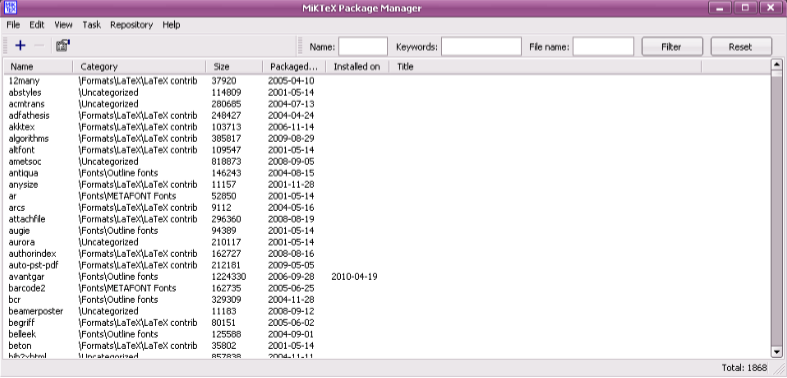
\includegraphics[width=12cm]{images/miktexpackage}
\end{center}

\end{frame}

\begin{frame}[fragile]
\frametitle{\textbf{Linux/Mac}}
\justifying
 \begin{block}{GNU/Linux}
Instalar el paquete: \texttt{latex-beamer}
\end{block}
\begin{block}{MacOSX}
Si descargaron MacTex completo no necesitan nada más.
\end{block}

\end{frame}
\subsection{Plantillas}
\begin{frame}[fragile]
\frametitle{\textbf{Plantillas}}
\justifying
 \begin{itemize}\justifying
  \item La forma más rápida de empezar a crear presentaciones es a partir de una plantilla.
  \item Plantillas disponibles en la web\footnote{\url{http://www.juaramir.com/latex/plantillas-latex}}.
  \item Descargar la plantilla e ir modificando cosas sobre ella.
  \item Compilar dos veces para ver el resultado final.
\end{itemize}

\end{frame}

\begin{frame}[fragile]
\frametitle{\textbf{Estructura Básica}}
\justifying
 \begin{itemize}\justifying
  \item La presentación empieza con \texttt{$\backslash$documentclass{beamer}}
  \item Información de preámbulo como en documentos normales\\(\texttt{usepackage}, \texttt{title}, \texttt{etc}).
  \item Contenido, con diferentes frames.
\end{itemize}

\begin{block}{}\small
$\backslash$\azul{documentclass}\{beamer\}\\
\verde{\%Preambulo}\\
$\backslash$\textbf{begin}\{document\}\\
$\backslash$\textbf{begin}\{frame\}\\
$\backslash$\textbf{frametitle}\{Primer Transparencia\}\\
\verde{\%Contenido}\\
$\backslash$\textbf{end}\{frame\}\\
$\backslash$\textbf{begin}\{frame\}\\
$\backslash$\textbf{frametitle}\{Segundo Transparencia\}\\
\verde{\%Contenido}\\
$\backslash$\textbf{end}\{frame\}\\
\%etc\\
$\backslash$\textbf{end}\{document\}\\
\end{block}




\end{frame}


\section{Elementos de la presentación}
\begin{frame}[fragile]
\frametitle{\textbf{Para Empezar}}
\justifying
 \begin{itemize}\justifying
  \item Crear una carpeta para guardar la presentación.
  \item Crea el documento básico que se muestra a continuación, y guárdalo en la carpeta recién creada.
\end{itemize}

$\backslash$\azul{documentclass}[utf8]\{beamer\}\\
$\backslash$\azul{usepackage}[spanish]\{babel\}\\
$\backslash$\textbf{usetheme}\{Warsaw\}\\
$\backslash$\textbf{begin}\{document\}\\\

$\backslash$\textbf{begin}\{frame\}\\
$\backslash$\textbf{frametitle}\{\}\\
\verde{\%Contenido}\\
$\backslash$\textbf{end}\{frame\}\\\

$\backslash$\textbf{end}\{document\}\\
\end{frame}

\begin{frame}[fragile]
\frametitle{\textbf{Resolución de la Presentación}}
\justifying
\begin{itemize}\justifying
  \item  Si deseamos cambiar el tamaño o dimensiones de la presentación para visualizar en pantallas widthscreen u otro formato, lo que debemos hacer es añadir el parámetro:\\ \texttt{aspectratio} al \texttt{documentclass}
  \item \texttt{$\backslash$documentclass[aspectratio=169]{beamer}}
  \item Si deseamos otras resoluciones debemos cambiar el \textbf{169} por: \textbf{1610}, \textbf{149}, \textbf{54}, \textbf{43} y \textbf{32}.
  \item Por defecto el valor es \textbf{43}.
\end{itemize}

\end{frame}

\subsection{Elementos Básicos}
\begin{frame}[fragile]
\frametitle{\textbf{Frames}}
\justifying
 Una presentación está compuesta por cuadros o frames, que a su vez generarán una o más diapositivas (\texttt{slides}), en función de si estamos usando efectos o no.
 
 \begin{exampleblock}{Un frame básico}
$\backslash$\textbf{begin}\{frame\}[fragile]\\
$\backslash$\textbf{frametitle}\{$\backslash$textbf\{Titulo del Frame\}\}\\\

 Contenido del Frame y Código $\backslash$LaTeX\{\}\\
$\backslash$\textbf{end}\{frame\}
\end{exampleblock}

 
\end{frame}

\begin{frame}[fragile]
\frametitle{\textbf{Opciones}}
\justifying
 
 \begin{description}\justifying
  \item [plain] oculta la barra de navegación. Deja más espacio para el contenido.
  \item [fragile] permite usar comandos que requieren protección, como \texttt{verbatim}.
  \item [b, c, t] define la alineación vertical.
  \item [label=nombre] asigna una etiqueta al frame.
  \item [allowframebreaks] divide el contenido en varios frames si es demasiado largo.
  \item [shrink] permite escribir mucho texto en una transparencia, reduciendo el tamaño de fuente según sea necesario.
\end{description}

 
\end{frame}

 \begin{frame}[fragile]
\frametitle{\textbf{Barra de Navegación}}
\justifying
 \begin{itemize}\justifying
  \item Se genera automáticamente.
  \item Dónde se sitúa y su aspecto dependen del tema que estemos usando.
  \item Contiene enlaces a las secciones y subsecciones (depende del tema).
\end{itemize}
\begin{center}

\includegraphics[width=12cm]{images/barra}
\end{center}

\end{frame}

\begin{frame}[fragile]
\frametitle{\textbf{Información del Documento}}
\justifying
 Para personalizar la presentación lo primero es cambiar los datos del documento.
 
\begin{exampleblock}{Información del Documento}

   \lstset{language=TEX}%SQL,basicstyle=\small}
   \vspace{-0.7cm}
\begin{lstlisting}
\title [título corto]{título largo}
\subtitle [subtítulo corto]{subtítulo largo}
\author [nombre corto]{nombre largo}
\date [fecha corta]{fecha larga}
\institute [nombre corto]{nombre largo}
\logo{\includegraphics[width=2cm]{images/logo.png}}
\end{lstlisting}\vspace{-0.3cm}
\end{exampleblock}
\end{frame}

\begin{frame}[fragile]
\frametitle{\textbf{Imagen de Fondo}}
\justifying

Se puede usar una imagen de fondo para la presentación (muy recomendable que sea semitransparente).

\begin{exampleblock}{Información del Documento}
   \lstset{language=TEX}%SQL,basicstyle=\small}
   \vspace{-0.7cm}
\begin{lstlisting}
\usebackgroundtemplate{
\includegraphics[width=\paperwidth, height=\paperheight]{images/fondo.png}
}
\end{lstlisting}\vspace{-0.3cm}

\end{exampleblock}
\end{frame}

\begin{frame}[fragile]
\frametitle{\textbf{Frame de Título}}
\justifying
 Se puede generar una diapositiva de título usando el comando $\backslash$titlepage.
 \begin{exampleblock}{Diapositiva de Título}
$\backslash$\textbf{begin}\{frame\}\\
$\backslash$titlepage\\
$\backslash$\textbf{end}\{frame\}\\

\end{exampleblock}

Si usamos la opción \texttt{[Plain]}, se ocultan las barras de navegación de la diapositiva.

 \begin{exampleblock}{Diapositiva de Título}
$\backslash$\textbf{begin}\{frame\}[plain]\\
$\backslash$titlepage\\
$\backslash$\textbf{end}\{frame\}\\
\end{exampleblock}
\end{frame}

\begin{frame}[fragile]
\frametitle{\textbf{Título de la Diapositiva}}
\justifying
 \begin{itemize}\justifying
  \item El título de la diapositiva se genera con el comando:
  \item []\texttt{$\backslash$frametitle[titulo corto]titulo largo}
  \item El título corto se utiliza cuando el largo ocupe demasiado, como puede pasar en el índice.
\end{itemize}
 \begin{exampleblock}{Diapositiva de Título}
$\backslash$\textbf{begin}\{frame\}\\
$\backslash$\textbf{frametitle}[titulo corto]\{titulo largo\}\\
$\backslash$framesubtitle\{subtitulo largo\}\\
$\backslash$\textbf{end}\{frame\}\\
\end{exampleblock}
\end{frame}

\begin{frame}[fragile]
\frametitle{\textbf{\centerline{Título de la Diapositiva}}}
\justifying
 Si se quiere centrar el título de la diapositiva hay que usar el comando \texttt{$\backslash$centerline\{\}}, del siguiente modo:
 
  \begin{exampleblock}{Título de la diapositiva centrados}
$\backslash$\textbf{begin}\{frame\}\\
$\backslash$\textbf{frametitle}[titulo corto]\{$\backslash$centerline\{titulo largo\}\}\\
$\backslash$\textbf{framesubtitle}\{subtitulo largo\}\\
$\backslash$\textbf{end}\{frame\}\\
\end{exampleblock}
\end{frame}

\begin{frame}[fragile]
\frametitle{\textbf{Tabla de contenidos}}
\justifying
 
 Se pueden generar tablas de contenidos usando el comando:\\ $\backslash$tableofcontents.
 \begin{exampleblock}{Tablas de Contenidos}
$\backslash$\textbf{begin}\{frame\}[plain]\\
$\backslash$frametitle\{Contenido\}\\
$\backslash$scriptsize \textit{\%para reducir el tama\~no de la letra}
$\backslash$\azul{tableofcontents}[pausesections]\\
$\backslash$\textbf{end}\{frame\}\\
\end{exampleblock}

\begin{itemize}\justifying
  \item La opción \texttt{pausesections} inserta una pausa en cada sección.
  \begin{itemize}\justifying
  \item []$\backslash$\azul{tableofcontents}[pausesections]
\end{itemize}

  \item La opción \texttt{currentsection} muestra la tabla de contenidos destacando la sección actual.
  \begin{itemize}\justifying
  \item []$\backslash$\azul{tableofcontents}[currentsection]\
\end{itemize}

\end{itemize}

 
\end{frame}

\begin{frame}[plain]
\frametitle{\textbf{Contenido con pausesections}}
\justifying
\scriptsize
 \tableofcontents[pausesections]
\end{frame}

\begin{frame}[plain]
\frametitle{\textbf{Contenido con currentsection}}
\justifying\scriptsize

 \tableofcontents[currentsection]
\end{frame}

\begin{frame}[fragile]
\frametitle{\textbf{Tabla de Contenidos}}
\justifying
 Generar automáticamente una tabla de contenido al principio de cada sección:
\begin{block}{}
   \lstset{language=TEX}%SQL,basicstyle=\small}
   \vspace{-0.7cm}
\begin{lstlisting}
\AtBeginSection[]
{\begin{frame}
\frametitle{Contenido}
\tableofcontents[currentsection]
\end{frame}}
\end{lstlisting}\vspace{-0.3cm}
\end{block}

\end{frame}

\begin{frame}[fragile]
\frametitle{\textbf{Tabla de Contenidos}}
\justifying
 Generar automáticamente una tabla de contenido al principio de cada subsección:
\begin{block}{}
   \lstset{language=}%SQL,basicstyle=\small}
   \vspace{-0.7cm}
\begin{lstlisting}
\AtBeginSection[]
{\begin{frame}
\frametitle{Contenido}
\tableofcontents[currentsection, currentsubsection]
\end{frame}}
\end{lstlisting}\vspace{-0.3cm}
\end{block}

\end{frame}

\begin{frame}[fragile]
\frametitle{\textbf{Tabla de Contenidos}}
\justifying
 \begin{itemize}\justifying
  \item Dividir automáticamente la tabla de contenidos en varios slides si ocupa demasiado espacio:
\end{itemize}
\begin{block}{}
   \lstset{language=}%SQL,basicstyle=\small}
   \vspace{-0.7cm}
\begin{lstlisting}
\tableofcontents[allowframebreaks]
\end{lstlisting}\vspace{-0.3cm}

\end{block}\begin{itemize}\justifying
  \item Por defecto después del título de diapositiva habrá un número romano (I, II, etc.).
  \item Para que sólo indique el número si hay mas de un slide:
\end{itemize}
\begin{block}{}
   \lstset{language=}%SQL,basicstyle=\small}
   \vspace{-0.7cm}
\begin{lstlisting}
\setbeamertemplate{frametitle continuation} % [from second] [\insertcontinuationcountroman]
\end{lstlisting}\vspace{-0.3cm}

\end{block}
\end{frame}


\begin{frame}[fragile]
\frametitle{\textbf{Subdivisión de la presentación}}
\justifying
 
 \begin{itemize}\justifying
  \item La presentación se puede dividir en partes (parts), secciones (sections), subsecciones (subsections) y subsubsecciones (subsubsections).
  \item Las secciones y subsecciones se mostrarán en la barra de navegación. Las partes permiten mostrar índices paciales.
\end{itemize}

\begin{exampleblock}{Generación de índices de una parte concreta}
   \lstset{language=}%SQL,basicstyle=\small}
   \vspace{-0.7cm}
\begin{lstlisting}
\tableofcontents[part=1]
\end{lstlisting}\vspace{-0.3cm}

\end{exampleblock}
\end{frame}

\subsection{Subdivisión de la presentación}
\begin{frame}[fragile]
\frametitle{\textbf{Subdivisión de la presentación}}
\justifying
 Hay que escribir estos comandos fuera de los frames, y hacen lo siguiente:
 \begin{itemize}\justifying
  \item Crean una entrada en la tabla de contenidos.
  \item Crean una entrada en la barra de navegación.
  \item NO crean el título de la diapositiva, eso hay que hacerlo con:
  \item [] \texttt{$\backslash$frametitle}.
\end{itemize}

La división modificada, con * (como \texttt{$\backslash$section*\{\}}) NO añade la entrada a la tabla de contenidos.
\end{frame}

\begin{frame}[fragile]
\frametitle{\textbf{Subdivisión del documento}}
\justifying
 \begin{block}{}
$\backslash$\azul{section}\{Introducci\'on\}\\
$\backslash$\azul{subsection}\{?`Qu\'e es beamer?\}\\
$\backslash$\textbf{begin}{frame}\\
$\backslash$\textbf{frametitle}\{Introducci\'on a beamer\}\\
Beamer es un paquete para la creaci\'on de presentaciones en $\backslash$LaTeX\{\}.\\
$\backslash$\textbf{end}\{frame\}\\
$\backslash$\azul{subsection}\{Instalaci\'on\}
\end{block}

\end{frame}

\subsection{Comandos \LaTeX{}}
\begin{frame}[fragile]
\frametitle{\textbf{Tipos de Letra}}
\justifying
 Se pueden utilizar todos los comandos normales de \LaTeX{}.
 
 \begin{minipage}[l]{0.60\linewidth}
   \lstset{language=}%SQL,basicstyle=\small}
   \vspace{-0.7cm}
\begin{lstlisting}
\emph{Texto de prueba}
\textbf{Texto de prueba}
\textit{Texto de prueba}
\textsl{Texto de prueba}
\alert{Texto de prueba}
\textrm{Texto de prueba}
\textsf{Texto de prueba}
\color{green} Texto de prueba
\structure{Texto de prueba}
\end{lstlisting}\vspace{-0.3cm}

\end{minipage}\hfill
\begin{minipage}[r]{0.38\linewidth}
\emph{Texto de prueba}\\
\textbf{Texto de prueba}\\
\textit{Texto de prueba}\\
\textsl{Texto de prueba}\\
\alert{Texto de prueba}\\
\textrm{Texto de prueba}\\
\textsf{Texto de prueba}\\
\color{green} Texto de prueba\\
\structure{Texto de prueba}
\end{minipage}

 
\end{frame}

\begin{frame}[fragile]
\frametitle{\textbf{Tamaños de Letra}}
\justifying
 \begin{minipage}[l]{0.55\linewidth}
   \lstset{language=,basicstyle=\small}
   \vspace{-0.7cm}
\begin{lstlisting}
\tiny{Texto tiny}
\scriptsize{Texto scriptsize}
\footnotesize{Texto footnotesize}
\small{Texto small}
\normalsize{Texto normalsize}
\large{Texto large}
\Large{Texto Large}
\LARGE{Texto LARGE}
\huge{Texto huge}
\Huge{Texto Huge}
\end{lstlisting}\vspace{-0.3cm}

\end{minipage}\hfill
\begin{minipage}[r]{0.44\linewidth}\vspace{-0.5cm}
\tiny{Texto tiny}\\\vspace{-0.5cm}
\scriptsize{Texto scriptsize}\\\vspace{-0.5cm}
\footnotesize{Texto footnotesize}\\\vspace{-0.5cm}
\small{Texto small}\\\vspace{-0.5cm}
\normalsize{Texto normalsize}\\\vspace{-0.5cm}
\large{Texto large}\\\vspace{-0.5cm}
\Large{Texto Large}\\\vspace{-0.2cm}
\LARGE{Texto LARGE}\\\vspace{-0.3cm}
\huge{Texto huge}\\\vspace{-0.1cm}
\Huge{Texto Huge}
\end{minipage}

\end{frame}

\begin{frame}[fragile]
\frametitle{\textbf{Comandos y Entornos \LaTeX{}}}
\justifying
 \begin{itemize}\justifying
  \item itemize
  \item enumerate
  \item description
  \item verse
  \item quote
  \item quotation
  \item footnote
  \item figure
  \item table
\end{itemize}

\end{frame}

\begin{frame}[fragile]
\frametitle{\textbf{Columnas}}
\justifying
 \begin{itemize}\justifying
  \item Se puede dividir el documento en varias columnas.
  \item En cada columna se puede poner texto, imágenes, tablas...
\end{itemize}

\begin{minipage}[l]{0.4\linewidth}


$\backslash$\textbf{begin}\{columns\} \\
$\backslash$\textbf{begin}\{column\}\{.4$\backslash$textwidth\} \\
Texto col 1.\\
$\backslash$\textbf{end}\{column\} \\
$\backslash$\textbf{begin}\{column\}\{.4$\backslash$textwidth\} \\
Texto col 2.\\
$\backslash$\textbf{end}\{column\}\\
$\backslash$\textbf{end}\{columns\}

\end{minipage}\hfill
\begin{minipage}[r]{0.58\linewidth}
\begin{columns} 
\begin{column}{.4\textwidth} 
Texto col 1.
\end{column} 
\begin{column}{.4\textwidth} 
Texto col 2.
\end{column}
\end{columns}
\end{minipage}

\end{frame}

\begin{frame}[fragile]
\frametitle{\textbf{Columnas}}
\justifying
 La división en columnas se puede hacer también usando el entorno \texttt{minipage}.
 
 \begin{minipage}[l]{0.48\linewidth}

$\backslash$\textbf{begin}\{minipage\}[l]\{0.48$\backslash$linewidth\}\\
Texto col 1.\\
$\backslash$\textbf{end}\{minipage\}$\backslash$hfill\\
$\backslash$\textbf{begin}\{minipage\}[r]\{0.48$\backslash$linewidth\}\\
Texto col 2.\\
$\backslash$\textbf{end}\{minipage\}

\end{minipage}\hfill
\begin{minipage}[r]{0.48\linewidth}
 \begin{minipage}[l]{0.48\linewidth}
Texto col 1.
\end{minipage}\hfill
\begin{minipage}[r]{0.48\linewidth}
Texto col 2.
\end{minipage}
\end{minipage}

 
\end{frame}

\begin{frame}[fragile]
\frametitle{\textbf{Texto Verbatim}}
\justifying
 \begin{itemize}\justifying
  \item Permite escribir texto o fórmulas tal y como se escriben, sin el formateo de \LaTeX{}.
  \item Esto se consigue de dos formas:
  \begin{itemize}\justifying
  \item Para texto dentro de una línea, como este \verb+\emph{Texto}+ se usa el comando $\backslash$verb+Texto+.
  \item Comando \texttt{verbatim}:
\end{itemize}
\begin{block}{}
$\backslash$\textbf{begin}\{verbatim\}\\
Formula mostrada textualmente \verb+$x^2$+\\
$\backslash$\textbf{end}\{verbatim\}
\end{block}

\item En cualquiera de los casos hay que definir el frame como frágil:
\item []$\backslash$begin\{frame\}[fragile].
\end{itemize}

\end{frame}

\begin{frame}[fragile]
\frametitle{\textbf{Texto con semiverbatim}}
\justifying
 
 \begin{itemize}\justifying
  \item Es como verbatim, pero ahora los comandos \rojo{$\backslash$}, \rojo{\{} y \rojo{\}} sí se interpretan.
  \item Esto permite, por ejemplo, formatear el texto.
  \item Para escribir un comando de forma textual hay que escribir dos barras (\rojo{$\backslash$$\backslash$}).
\end{itemize}
\begin{exampleblock}{Ejemplo}
$\backslash$\textbf{begin}\{semiverbatim\}\\
  Texto $\backslash$\rojo{alert}\{no\} interpretado. He usado el comando $\backslash$$\backslash$alert\\
$\backslash$\textbf{end}\{semiverbatim\}
\end{exampleblock}

\begin{block}{Resultado}
\begin{semiverbatim}
  Texto \alert{no} interpretado. He usado el comando \\alert
\end{semiverbatim}
\end{block}
\end{frame}
\subsubsection{Otros entornos}
\begin{frame}[fragile]
\frametitle{\textbf{Otros entornos}}
\justifying
 \begin{itemize}\justifying
  \item equation
  \item theorem
  \item proof
\end{itemize}

\end{frame}

\begin{frame}[fragile]
\frametitle{\textbf{Equation}}
\justifying
 \begin{block}{}
$\backslash$\textbf{begin}\{equation\}\\
u(x)=\\
$\backslash$\textbf{begin}\{cases\}\\
$\backslash$exp\{x\}    \& $\backslash$text\{if \} x $\backslash$geq 0$\backslash$$\backslash$\\
 1 \& $\backslash$text\{if \} x $<$ 0\\
 $\backslash$\textbf{end}\{cases\}\\
$\backslash$\textbf{end}\{equation\}

\end{block}
\begin{equation}
u(x)=
\begin{cases}
\exp{x}    & \text{if } x \geq 0\\
 1 & \text{if } x < 0
 \end{cases}
\end{equation}
\end{frame}

\begin{frame}[fragile]
\frametitle{\textbf{Theorem}}
\justifying
 \begin{itemize}\justifying
  \item En una presentación crea un bloque que contiene la definición.
  \item Requiere el paquete \texttt{amsthm}.
\end{itemize}

\begin{block}{}
$\backslash$\textbf{newtheorem}\{midef\}\{Definición\}\\
$\backslash$\textbf{begin}\{midef\}\\
Esto es una definición.    \\
$\backslash$\textbf{end}\{midef\}
\end{block}

\newtheorem{midef}{Definición}
\begin{midef}
Esto es una definición.    
\end{midef}
\end{frame}

\begin{frame}[fragile]
\frametitle{\textbf{Proof}}
\justifying
 \begin{block}{}
$\backslash$\textbf{begin}\{proof\}[Demostración del Teorema]\\
    Esta es la demostración:\\
    $\backslash$[ \verb+a^2+ + \verb+b^2+ = \verb+c^2+ $\backslash$qedhere $\backslash$]\\
$\backslash$\textbf{end}\{proof\}
\end{block}
\begin{proof}[Demostración del Teorema]
    Esta es la demostración:
    \[ a^2 + b^2 = c^2 \qedhere \]
\end{proof}
\end{frame}
\subsubsection{Bloques}
\begin{frame}[fragile]
\frametitle{\textbf{Bloque}}
\justifying
 \begin{itemize}\justifying
  \item Existen 3 comandos para dibujar bloques: \texttt{block}, \texttt{alertblock} y \texttt{exampleblock}.
\end{itemize}

$\backslash$begin\{block\}\{Título del bloque\}\\
Contenido del bloque\\
$\backslash$end\{block\}

\begin{block}{Título del bloque}
Contenido del bloque
\end{block}


\end{frame}


\begin{frame}[fragile]
\frametitle{\textbf{Bloque de alerta}}
\justifying
 $\backslash$\textbf{begin}\{alertblock\}\{Título del bloque\}\\
Contenido del bloque\\
$\backslash$\textbf{end}\{alertblock\}

\begin{alertblock}{Título del bloque}
Contenido del bloque
\end{alertblock}

\end{frame}

\begin{frame}[fragile]
\frametitle{\textbf{Bloque de ejemplo}}
\justifying
 $\backslash$\textbf{begin}\{exampleblock\}\{Título del bloque\}\\
Contenido del bloque\\
$\backslash$\textbf{end}\{exampleblock\}

\begin{exampleblock}{Título del bloque}
Contenido del bloque
\end{exampleblock}

\end{frame}

\section{Temas}
\begin{frame}[fragile]
\frametitle{\textbf{Tipos de Temas}}
\justifying
 La apariencia de las trasparencias se define mediante temas.
\begin{description}\justifying
  \item[Globales] Controlan la apariencia global. \texttt{$\backslash$usetheme}
  \item[Color] Permiten cambiar el color. \texttt{$\backslash$usecolortheme}.
  \item[Fuentes] Personalizan las fuentes. \texttt{$\backslash$usefonttheme}
  \item[Internos] Cambian el aspecto interno. \texttt{$\backslash$useinnertheme}
  \item[Externos] Aspectos externos. \texttt{$\backslash$useroutertheme}
\end{description}
\begin{itemize}\justifying
  \item La guía de usuario Beamer\footnote{J. Wright, V. Mleti\'c. The beamer class. \url{http://www.ctan.org/tex-archive/macros/latex/contrib/beamer/doc/ beameruserguide.pdf}} contiene información detallada sobre diferentes temas, las opciones que tienen y el aspecto final.
\end{itemize}

\end{frame}

\subsection{Temas Globales}
\begin{frame}[fragile]
\frametitle{\textbf{Temas sin barra de navegación}}
\justifying
 \begin{itemize}\justifying
  \item Bergen
  \item Madrid
  \item AnnArbor
  \item Rochester
  \item JuanLesPins
  \item Montpellier
\end{itemize}
\begin{block}{Ejemplo}
$\backslash$usetheme\{Montpellier\}
\end{block}
\end{frame}

\begin{frame}[fragile]
\frametitle{\textbf{Temas con barra de navegación lateral}}
\justifying
 \begin{itemize}\justifying
  \item Berkeley
  \item PaloAlto
  \item Goettingen
  \item Marburg
\end{itemize}
\begin{block}{Ejemplo}
$\backslash$usetheme\{Marburg\}
\end{block}
\end{frame}

\begin{frame}[fragile]
\frametitle{\textbf{Temas con margo de navegación}}
\justifying
 \begin{itemize}\justifying
  \item Berlin
  \item Dresden
  \item Darmstadt
  \item  Frankfurt
  \item Singapore
  \item Szeged
\end{itemize}
\begin{block}{Ejemplo}
$\backslash$usetheme\{Szeged\}
\end{block}
\end{frame}

\begin{frame}[fragile]
\frametitle{\textbf{Temas con tabla de sección y subsecciones}}
\justifying
 \begin{itemize}\justifying
  \item Copenhagen
  \item Luebeck
  \item Warsaw
\end{itemize}

\begin{block}{Ejemplo}
$\backslash$usetheme\{Warsaw\}
\end{block}


\end{frame}

\subsection{Temas de Color}

\begin{frame}[fragile]
\frametitle{\textbf{Temas de Color}}
\justifying
 Los temas de color se especifican con \texttt{$\backslash$usecolortheme\{\}}
 
 \begin{itemize}\justifying
  \item albatross
  \item beaver
  \item beetle
  \item crane
  \item default
  \item dolphin
  \item$\dots$
  \item seahorse (colores suaves)
  \item etc.
\end{itemize}
\begin{block}{}
\begin{itemize}\justifying
  \item Visita la pagina:
  \item []\url{https://www.hartwork.org/beamer-theme-matrix/} y comprueba las diferentes combinaciones de temas globales y temas de color.
  \item Elige una combinación y utilizala.
\end{itemize}

\end{block}

\end{frame}

\begin{frame}[fragile]
\frametitle{\textbf{Tema de color structure}}
\justifying
 \begin{itemize}\justifying
  \item Podemos definir el color por su nombre usando la opción:
  \item [] \texttt{dvipsnames} del paquete \texttt{xcolor}, así:
  \item [] \texttt{$\backslash$documentclass[xcolor=dvipsnames]\{beamer\}}
  \item Algunos colores:
  \begin{itemize}\justifying
  \item Peach
  \item Orange
  \item Bittersweet
  \item Mahogany
  \item Periwinkle
  \item etc.
\end{itemize}
\item[] \texttt{
$\backslash$usecolortheme[named=Mahogany]\{structure\}}
\item Consulta colores disponibles en:\\
\url{http://tex.loria.fr/graph-pack/grf/grf.pdf} (en la última pagina).
\end{itemize}

\end{frame}


\begin{frame}[fragile]
\frametitle{\textbf{Tema de color structure}}
\justifying
\begin{itemize}\justifying
  \item Además de los colores predefinidos, se pueden utilizar otros tonos para structure.
  \item [] \texttt{$\backslash$usecolortheme\rojo{[RGB=\{148,20,110\}]}\{structure\}}
  \item Se especifica el color mediante sus componentes R, G y B.
\end{itemize}
\end{frame}


\subsection{Temas Externos}
\begin{frame}[fragile]
\frametitle{\textbf{Temas Externos}}
\justifying
 \begin{itemize}\justifying
  \item Un tema externo (outer theme) define cómo se muestran los siguientes elementos:
  \begin{itemize}\justifying
  \item Encabezado y pie de diapositiva.
  \item Barras laterales, si las hubiera.
  \item Logo.
  \item Título de diapositiva.
  \item Barra de navegación.
\end{itemize}

\end{itemize}

\end{frame}

\begin{frame}[fragile]
\frametitle{\textbf{Temas Externos}}
\justifying
 \begin{itemize}\justifying
  \item Comando \texttt{$\backslash$useoutertheme\{nombreTema\}}
  \item Temas disponibles:
  \begin{itemize}\justifying
  \item default
  \item infolines
  \item miniframes
  \item sidebar
  \item split
  \item shadow
  \item tree
  \item smoothtree
\end{itemize}

\end{itemize}

\end{frame}

\subsection{Temas Internos}
\begin{frame}[fragile]
\frametitle{\textbf{Temas Internos}}
\justifying
 \begin{itemize}\justifying
  \item Un tema interno (inner theme) define cómo se muestran los siguientes elementos:
  \begin{itemize}\justifying
  \item Página de portada.
  \item Entornos de listas (numeradas, no numeradas, descripción).
  \item Entornos de bloques.
  \item Entornos de theorem y proof.
  \item Figuras y tablas.
  \item Pies de página.
  \item Entradas bibliográficas.
\end{itemize}

\end{itemize}

\end{frame}

\begin{frame}[fragile]
\frametitle{\textbf{Temas Internos}}
\justifying
 \begin{itemize}\justifying
  \item Comando \texttt{$\backslash$useinnertheme\{nombreTema\}}
  \item Temas disponibles:
  \begin{itemize}\justifying
  \item default.
  \item circles.
  \item rectangles.
  \item rounded.
  \item inmargin.
\end{itemize}

\end{itemize}

\end{frame}


\section{Efectos}
\subsection{Overlays}
\begin{frame}[fragile]
\frametitle{\textbf{Introducción}}
\justifying
 \begin{itemize}\justifying
  \item Un overlay permite ir mostrando diferentes cosas en el mismo frame.
  \item En realidad, en el archivo pdf tendremos varias páginas (slides).
  \item Da la impresión de que vamos añadiendo elementos a una misma página.
  \item Podemos generar un documento para su impresion que ignora los overlays usando la opción handout de la clase beamer.
  \item []\texttt{$\backslash$documentclass\rojo{[handout]}\{beamer\}}
\end{itemize}

\end{frame}

\subsubsection{Pause}
\begin{frame}[fragile]
\frametitle{\textbf{Lista elemento a elemento (pause)}}
\justifying
 \begin{itemize}\justifying
  \item El comando a usar es \texttt{$\backslash$pause}
  \item Permite mostrar la transparencia por pasos.
  \item Solo muestra el texto que hay antes de esta instrucción.
  \item El texto que lo sigue se mostrará en la siguiente transparencia.
  \item El texto no mostrado aparece en claro.
\end{itemize}

\end{frame}

\begin{frame}[fragile]
\frametitle{\textbf{Lista elemento a elemento (pause)}}
\justifying
 \begin{itemize}\justifying
  \item Podemos usar el comando \texttt{$\backslash$pause} para ir mostrando los elementos uno a uno.
  \pause \item Como en este ejemplo.
  \pause \item Evita que la audiencia se distraiga.
\end{itemize}

\begin{exampleblock}{Código}
 $\backslash$\textbf{begin}\{itemize\}\\
  $\backslash$item Podemos usar el comando $\backslash$texttt\{$\backslash$pause\} para ir mostrando los elementos uno a uno.\\
  $\backslash$\textbf{pause} $\backslash$item Como en este ejemplo.\\
  $\backslash$\textbf{pause} $\backslash$item Evita que la audiencia se distraiga.\\
$\backslash$\textbf{end}\{itemize\}
\end{exampleblock}

\end{frame}

\subsubsection{$\backslash$item$<$n-$>$}
\begin{frame}[fragile]
\frametitle{\textbf{Lista elemento a elemento ($\backslash$item$<$n-$>$)}}
\justifying
 \begin{itemize}\justifying
  \item Método alternativo para mostrar elementos por pasos.
  \item Permite indicar a partir de qué elemento queremos que se muestre.
  \item También se puede especificar un intervalo:
  \item [] \texttt{$<$n-$>$}, \texttt{$<$n-m$>$}, \texttt{$<$n$>$}, \texttt{$<$n,m$>$}.
  \item El siguiente ejemplo muestra cómo se puede definir la visualización.
\end{itemize}

\end{frame}

\begin{frame}[fragile]
\frametitle{\textbf{Lista elemento a elemento ($\backslash$item$<$n-$>$)}}
\justifying
 \begin{itemize}
\item<2-> Aparece a partir del slide 2.
 \item<2-4> Aparece del slide 2 al 4. 
 \item<2,4> Aparece en los slides 2 y 4. 
 \item<-3> Aparece hasta el slide 3. 
\end{itemize}  
 
\begin{exampleblock}{Código}
$\backslash$begin\{itemize\}\\
$\backslash$item$<$2-$>$ Aparece a partir del slide 2.\\
 $\backslash$item$<$2-4$>$ Aparece del slide 2 al 4. \\
 $\backslash$item$<$2,4$>$ Aparece en los slides 2 y 4.\\ 
$\backslash$item$<$-3$>$ Aparece hasta el slide 3. \\
$\backslash$end\{itemize\}    
\end{exampleblock}


\end{frame}

\subsubsection{Mostrar y Olcultar}
\begin{frame}[fragile]
\frametitle{\textbf{Mostrar y Ocultar ($\backslash$uncover)}}
\justifying
 \texttt{$\backslash$uncover$<$slides$>$\{Texto\}}
 \begin{itemize}\justifying
  \item En la opción \texttt{$<$slides$>$} podemos indicar \texttt{$<$n-$>$}, \texttt{$<$n-m$>$}, \texttt{$<$n$>$}, \texttt{$<$n,m$>$}.
  \item A continuación se muestra un ejemplo del funcionamiento de este comando.
  \item No solo sirve para items de listas: también para figuras, columnas, etc.
\end{itemize}

\end{frame}

\begin{frame}[fragile]
\frametitle{\textbf{Mostrar y Ocultar ($\backslash$uncover)}}
\justifying
 
\uncover<-2>{Hasta el slide 2\\}
\uncover<2->{A partir del slide 2\\}
\uncover<3-4>{Del slide 2 al 4\\}
\uncover<4>{En el slide 4\\} 
\uncover<3->{A partir del slide 3\\}
 
\begin{exampleblock}{Código}
$\backslash$uncover$<$-2$>$\{Hasta el slide 2$\backslash$$\backslash$\}\\
$\backslash$uncover$<$2-$>$\{A partir del slide 2$\backslash$$\backslash$\}\\
$\backslash$uncover$<$3-4$>$\{Del slide 2 al 4$\backslash$$\backslash$\}\\
$\backslash$uncover$<$4$>$\{En el slide 4$\backslash$$\backslash$$\backslash$\} \\
$\backslash$uncover$<$3-$>$\{A partir del slide 3$\backslash$$\backslash$\}
\end{exampleblock}

 
\end{frame}

\begin{frame}[fragile]
\frametitle{\textbf{Mostrar y Ocultar ($\backslash$only)}}
\justifying
  \texttt{$\backslash$only$<$slides$>$\{Texto\}}
 \begin{itemize}\justifying
  \item En la opción \texttt{$<$slides$>$} podemos indicar \texttt{$<$n-$>$}, \texttt{$<$n-m$>$}, \texttt{$<$n$>$}, \texttt{$<$n,m$>$}.
  \item Funciona como \texttt{$\backslash$uncover} pero no reserva sitio para los elementos que aún no se muestran.
  \item A continuación se muestra un ejemplo del funcionamiento de este comando.
  \item No solo sirve para items de listas: también para figuras, columnas, etc.
\end{itemize}

\end{frame}

\begin{frame}[fragile]
\frametitle{\textbf{Mostrar y Ocultar ($\backslash$only)}}
\justifying
 
\only<-2>{Aparece hasta el slide 2\\} 
\only<2->{Aparece a partir del slide 2\\}
\only<3-4>{Aparece del slide 3 al 4\\}
\only<4>{Aparece en el slide 4 4\\}
\only<3->{Aparece a partir del slide 3\\}
 
\begin{exampleblock}{Código}
$\backslash$only$<$-2$>$\{Aparece hasta el slide 2$\backslash$$\backslash$\} \\
$\backslash$only$<$2-$>$\{Aparece a partir del slide 2$\backslash$$\backslash$\}\\
$\backslash$only$<$3-4$>$\{Aparece del slide 3 al 4$\backslash$$\backslash$\}\\
$\backslash$only$<$4$>$\{Aparece en el slide 4$\backslash$$\backslash$\}\\
$\backslash$only$<$3-$>$\{Aparece a partir del slide 3$\backslash$$\backslash$\}\\
\end{exampleblock}

\end{frame}

\begin{frame}[fragile]
\frametitle{\textbf{Mostrar y Ocultar ($\backslash$invisible)}}
\justifying
   \texttt{$\backslash$invisible$<$slides$>$\{Texto\}}
 \begin{itemize}\justifying
  \item En la opción \texttt{$<$slides$>$} podemos indicar \texttt{$<$n-$>$}, \texttt{$<$n-m$>$}, \texttt{$<$n$>$}, \texttt{$<$n,m$>$}.
  \item Funciona como \texttt{$\backslash$uncover} pero hace que el texto sea invisible en los slides indicados. 
  \item A continuación se muestra un ejemplo del funcionamiento de este comando.
  \item No solo sirve para items de listas: también para figuras, columnas, etc.
\end{itemize}
\end{frame}

\begin{frame}[fragile]
\frametitle{\textbf{Mostrar y Ocultar ($\backslash$invisible)}}
\justifying
 
 \invisible<2>{Este texto será invisible en el slide 2.}\\ Este texto siempre será visible\\
 
 \begin{exampleblock}{Código}
 $\backslash$invisible$<$2$>$\{Este texto será invisible en el slide 2.\}$\backslash$$\backslash$\\
 Este texto siempre será visible$\backslash$$\backslash$
\end{exampleblock}

 
\end{frame}

\begin{frame}[fragile]
\frametitle{\textbf{Otros comandos para overlays}}
\justifying
\begin{description}\justifying
  \item[$\backslash$alt$<$slide$>$\{Texto1\}\{Texto2\}] Muestra Texto1 en los slides indicados y Texto2 en el resto.
  \item[$\backslash$alert$<$slide$>$Texto] Muestra el Texto en forma de alerta (rojo).
  \item[$\backslash$color$<$slide$>$colortexto] Muestra el texto en el color indicado.
\end{description}
\end{frame}

\begin{frame}[fragile]
\frametitle{\textbf{Otros comandos para overlays}}
\justifying
 Hay otros comandos que permiten especificar a qué transparencia deben aplicarse.
 \begin{itemize}\justifying
  \item $\backslash$textbf
  \item $\backslash$textit
  \item $\backslash$textsl
  \item $\backslash$textrm
  \item $\backslash$textsf
  \item structure
\end{itemize}

\end{frame}


\subsubsection{Mostrar Tablas Dinámicamente}
\begin{frame}
\frametitle{\textbf{Mostrar Filas Dinámicamente}}
\justifying
 \begin{itemize}\justifying
  \item Incluir el paquete \texttt{colortbl}
  \item Usar el comando $\backslash$pause
\end{itemize}

\begin{center}
\begin{tabular}{lcccc} 
Class&A&B&C&D \\\hline 
 X &1&2&3&4 \pause\\ 
Y &3&4&5&6 \pause\\
Z &5&6&7&8\\
\end{tabular}
\end{center}

\begin{exampleblock}{Código}
$\backslash$begin\{tabular\}\{lcccc\} 
Class\&A\&B\&C\&D $\backslash$$\backslash$$\backslash$hline \\
 X \&1\&2\&3\&4 $\backslash$pause$\backslash$$\backslash$\\ 
Y \&3\&4\&5\&6 $\backslash$pause$\backslash$$\backslash$\\
Z \&5\&6\&7\&8$\backslash$$\backslash$\\
$\backslash$end\{tabular\}
\end{exampleblock}

\end{frame}
\begin{frame}
\frametitle{\textbf{Mostrar Columnas Dinámicamente}}
\justifying
 \begin{itemize}\justifying
  \item Incluir el paquete \texttt{colortbl}
  \item Usar el comando $\backslash$onslide
\end{itemize}

\begin{center}
\begin{tabular}{l|c<{\onslide<2->}|c<{\onslide<3->}|c<{\onslide<4->}|c<{\onslide}|c}
Clase & A & B & C & D \\ 
X & 1 & 2 & 3 & 4 \\ 
Y & 3 & 4 & 5 & 6 \\ 
Z &5&6&7&8 
\end{tabular}
\end{center}

\begin{exampleblock}{Código}
$\backslash$begin\{tabular\}\{l|c$<$\{$\backslash$onslide$<$2-$>$\}|c$<$\{$\backslash$onslide$<$3-$>$\}|c$<$\{$\backslash$onslide$<$4-$>$\}|c$<$\{$\backslash$onslide\}|c\}\\
Clase \& A \& B \& C \& D $\backslash$$\backslash$\\ 
X \& 1 \& 2 \& 3 \& 4 $\backslash$$\backslash$\\ 
Y \& 3 \& 4 \& 5 \& 6 $\backslash$$\backslash$\\ 
Z \&5\&6\&7\&8 
$\backslash$end\{tabular\}
\end{exampleblock}

\end{frame}

\subsection{Transiciones}
\begin{frame}[fragile]
\frametitle{\textbf{Tipos de transiciones entre diapositivas}}
\justifying
 A pesar de que el archivo sea un PDF, se pueden definir transiciones:
 \begin{itemize}\justifying
  \item $\backslash$transblindshorizontal
  \item $\backslash$transblindsvertical
  \item $\backslash$transboxin
  \item $\backslash$transboxout
  \item $\backslash$transdissolve
  \item $\backslash$transglitter
  \item $\backslash$transsplithorizontalin
  \item $\backslash$transsplithorizontalout
  \item $\backslash$transsplitverticalin
  \item $\backslash$transsplitverticalout
  \item $\backslash$transwipe
\end{itemize}

\end{frame}
\transdissolve

\subsection{Botones y Enlaces Internos}
\begin{frame}[fragile]
\frametitle{\textbf{Tipos de Botones}}
\justifying
 \begin{description}\justifying
  \item[$\backslash$beamergotobutton texto] Crea un botón con el texto indicado. El símbolo es una flecha que indica que al hacer clic se salta a otra zona de la presentación.
  \item[$\backslash$beamerskipbutton texto] Crea un botón con dos flechas que al pulsarlo se salta parte de la presentación.
  \item[$\backslash$beamerreturnbutton texto] Botón con una flecha hacia la izquierda. Al pulsarlo se vuelve a una parte anterior de la presentación.
\end{description}
Para más información, consultar el manual de beamer.
\end{frame}

\subsection{Zoom en Imágenes}
\begin{frame}[fragile]
\frametitle{\textbf{Haciendo Zoom en Imágenes}}
\justifying
 \begin{itemize}\justifying
  \item Se puede hacer zoom en imágenes usando:
  \item [] $\backslash$framezoom$<$slide origen$><$slide zoom$>$(x,y)(w,h)
  \begin{description}\justifying
  \item[slide origen] Indica en qué slide está la imagen completa.
  \item[slide zoom] Indica en qué slide estará la imagen ampliada.
  \item[(x,y)] Origen de la imagen a ampliar (punto superior izquierdo).
  \item[(w,h)] Tamaño del área a ampliar.
\end{description}

\end{itemize}

\end{frame}


\begin{frame}[fragile]
\frametitle{\textbf{Zoom en Imágenes}}
\justifying
\framezoom<1><2>[border](0.3\textwidth,1cm)(3cm,2cm)
\framezoom<1><3>[border](0.4\textwidth,3.5cm)(2cm,1.5cm)
\framezoom<1><4>[border](0.5\textwidth,3cm)(2cm,2cm)
\begin{center}

\includegraphics[width=0.6\textwidth]{images/wallpaper-1920.jpg} \end{center}
\end{frame}

\begin{frame}[fragile]
\frametitle{\textbf{Zoom en Imágenes}}
\justifying
 \begin{block}{Código}
$\backslash$framezoom$<$1$><$2$>$[border](0.3$\backslash$textwidth,1cm)(3cm,2cm) \\
$\backslash$framezoom$<$1$><$3$>$[border](0.4$\backslash$textwidth,3.5cm)(2cm,1.5cm)\\
$\backslash$framezoom$<$1$><$4$>$[border](0.5$\backslash$textwidth,3cm)(2cm,2cm) \\
$\backslash$begin\{center\}\\
$\backslash$includegraphics[width=0.6$\backslash$textwidth]\{images/wallpaper-1920.jpg\}\\
$\backslash$end\{center\}
\end{block}

\end{frame}


\section{Bibliografía}
\begin{frame}[fragile]
\frametitle{\textbf{Inclusión de Bibliografía}}
\justifying
 \begin{itemize}\justifying
  \item Se puede incluir bibliografía usando $\backslash$thebibliography, como en \LaTeX{}.
  \item \texttt{beamer} dispone de plantillas para mostrar las bibliografías de artículos y libros de forma más agradable.
  \item Se llaman con:
  \begin{itemize}\justifying
  \item Libros: \texttt{$\backslash$beamertemplatebookbibitems}
  \item Articulos: \texttt{$\backslash$beamertemplatearticlebibitems}
\end{itemize}
  \item A continuación se muestra el código utilizado para generar la bibliografía de esta presentación.
\end{itemize}
\end{frame}

\begin{frame}[fragile]
\frametitle{\textbf{Inclusión de Bibliografía}}
\justifying

$\backslash$\textbf{begin}\{frame\}[allowframebreaks]\\
$\backslash$frametitle\{Referencias\} \\
$\backslash$\textbf{begin}\{thebibliography\}\{10\}\\
$\backslash$beamertemplatebookbibitems\\
$\backslash$bibitem\{Tantau2010\}J.Wright., V. Mleti\'c\\
$\backslash$newblock \{$\backslash$em The beamer class\}.\\
$\backslash$newblock $\backslash$\textbf{begin}\{scriptsize\} $\backslash$url\{\url{http://goo.gl/iTHpOa}\}.\\
$\backslash$\textbf{end}\{scriptsize\}\\
$\backslash$beamertemplatearticlebibitems \\
$\backslash$bibitem\{Batts2007\}C. T. Batts\\
$\backslash$newblock A Beamer Tutorial in Beamer. $\backslash$newblock $\backslash$\textbf{begin}\{scriptsize\} 
$\backslash$url\{\url{http://goo.gl/3rrKQ6}\}.$\backslash$\textbf{end}\{scriptsize\}\\
$\backslash$\textbf{end}\{thebibliography\}\\
$\backslash$\textbf{end}\{frame\}

\end{frame}


\begin{frame}[allowframebreaks]
\frametitle{Referencias} 
\begin{thebibliography}{10}
\beamertemplatebookbibitems
\bibitem{Tantau2010}J.Wright. , V. Mleti\'c
\newblock {\em The beamer class}.
\newblock \begin{scriptsize} \url{http://goo.gl/iTHpOa}.\end{scriptsize}
\beamertemplatearticlebibitems 
\bibitem{Batts2007}C. T. Batts
\newblock A Beamer Tutorial in Beamer . \newblock \begin{scriptsize} \url{http://goo.gl/3rrKQ6}.
\end{scriptsize}
\end{thebibliography}
\end{frame}

\end{document}